\section{Registers}
\label{sec:registers}

Circuits that include flip-flops are usually classified by the function they perform rather than by the name of the sequential circuit. Two such circuits are \textit{registers} and \textit{counters}.
\begin{itemize}[leftmargin=0.7cm]
  \item A \textbf{register} is a \textit{group of flip-flops}, each one of which shares a common clock and is capable of storing one bit of information. An $n$-bit register consists of a group of $n$ flip-flops capable of storing $n$ bits of binary information. In addition to the flip-flops, a register may have combinational gates that perform certain data-processing tasks. 

  In its broadest definition, a register consists of a group of flip-flops together with gates that affect their operation. The flip-flops hold the binary information, and the gates determine how the information is transferred into the register.

  \item A \textbf{counter} is essentially \textit{a register that goes through a predetermined sequence of binary states}. The gates in the counter are connected in such a way as to produce the prescribed sequence of states. Although counters are a special type of register, it is common to differentiate them by giving them a different name.
\end{itemize}

\noindent The simplest register is one that consists of only flip-flops, without any gates. Figure 1 shows such a register constructed with four $D$-type flip-flops to form a four-bit data storage register.


\subsection{Register with Parallel Load}
\label{subsec:register-with-parallel-load}

Registers with parallel load are a fundamental building block in digital systems. Synchronous digital systems have a master clock generator that supplies a continuous train of clock pulses. The pulses are applied simultaneously to all flip-flops and registers in the system. A separate control signal must be used to decide which register operation will execute at each clock pulse. The transfer of new information into a register is referred to as \textit{loading} or \textit{updating} the register. 

If all the bits of the register are loaded simultaneously with a common clock pulse, we say that the loading is done in \textit{parallel}. A clock edge applied to the $C$ inputs of the register of Fig. 1 will load all four inputs in parallel. In this configuration, if the contents of the register must be left unchanged, the inputs must be held constant or the clock must be inhibited from the circuit.
\begin{itemize}[leftmargin=0.7cm]
  \item In the first case, the data bus driving the register would be unavailable for other traffic.
  \item In the second case, the clock can be inhibited from reaching the register by controlling the clock input signal with an enabling gate.
\end{itemize}
\noindent However, inserting gates into the clock path is ill-advised because it means that logic is performed with clock pulses. The insertion of logic gates in the path of the clock signal produces uneven propagation delays between the master clock and the inputs of flip-flops.

A four-bit data-storage register with a load control input that is directed through gates and into the $D$ inputs of the flip-flops is shown in Fig. 2. The additional gates implement a two-channel mux whose output drives the input to the register with either the data bus or the output of the register. The \textit{load} input to the register determines the action to be taken with each clock pulse. When the \textit{load} input is 1, the data at the four external inputs are transferred into the register with the next positive edge of the clock. When the \textit{load} input is 0, the outputs of the flip-flops are connected to their respective inputs.
\begin{figure}[H]
  \centering
  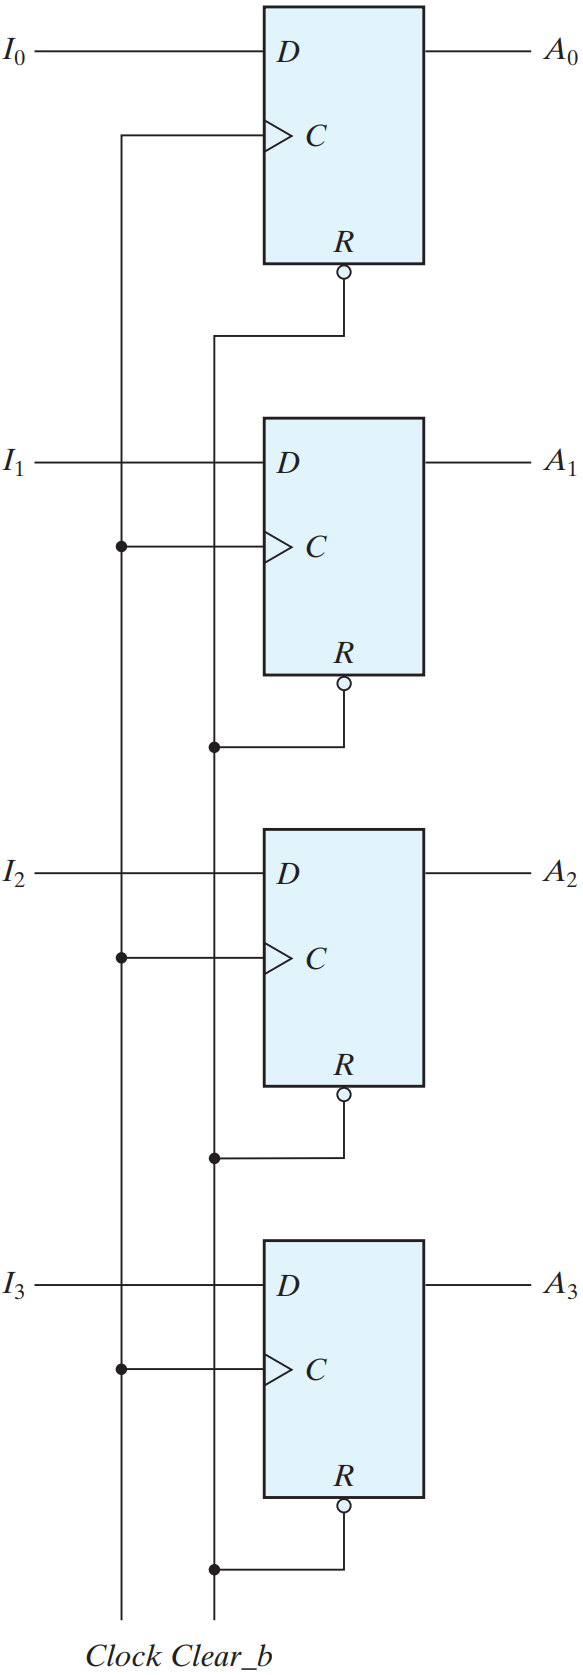
\includegraphics[width=.7\linewidth]{img/fig-6.1.png}
  \caption{Four-bit register}
  \label{fig:6.1}
\end{figure}

\begin{figure}[H]
  \centering
  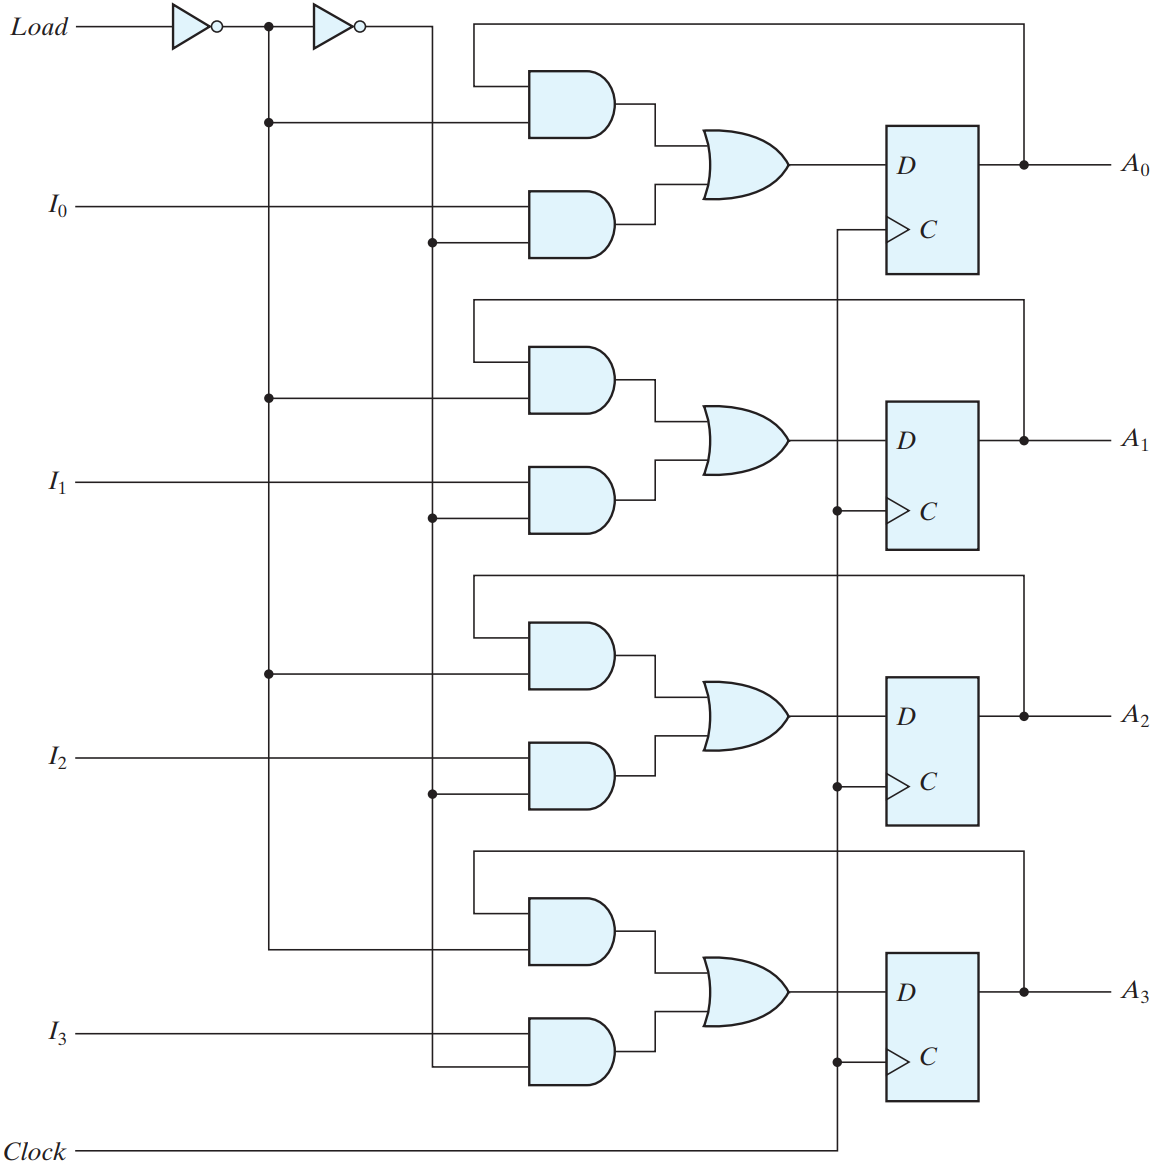
\includegraphics[width=\linewidth]{img/fig-6.2.png}
  \caption{Four-bit register with parallel load}
  \label{fig:6.2}
\end{figure}
